%!TEX root = ../main.tex
\section{Semantic Routing in the Fog}
\label{sec:semantic-routing-in-the-fog}

In this section we adapt Semantic Routing Trees from TinyDB for a use in the fog. We first explain the differences in target environments that necessitate reassessing the design of SRTs (Section~\ref{Differences in Target Environments}). From there, we succinctly describe our view on the potential use cases for SRTs in Section~\ref{Applications of Semantic Routing Trees in the Fog}. Afterwards, we conceptually adapt SRTs based on the environmental differences in Section~\ref{Adaption of Semantic Routing Trees to the Fog}. Because we identify the choice of which remote nodes a node should track as critical for performance, we conclude the section with the description of a node-tracking policy in Section~\ref{Node-Tracking Policies}. Lastly, we examine the tree construction and maintenance process in Section~\ref{Tree Construction and Maintenance}

\section{Differences in Target Environments}\label{Differences in Target Environments}
  \bgroup % For vertical padding
  \def\arraystretch{1.25}
  \begin{table}
    \begin{tabular}{l|l|l}
      & \textbf{Wireless Sensor} & \textbf{Fog Layer} \\
      & \textbf{Networks} & \\
      \hline
      \textbf{Computational} & \textbullet~Homogenous & \textbullet~Heterogenous \\
      \textbf{power} & \textbullet~Very low & \textbullet~Varying \\
      \hline
      \textbf{Energy supply} & \textbullet~Battery & \textbullet~Battery and grid  \\
      \hline
      \textbf{Connectivity} & \textbullet~Wireless &  \textbullet~Wireless and wired\\
      && \textbullet~Internet connection \\
      \hline
      \textbf{Hardware architectures} & \textbullet~Homogenous & \textbullet~Heterogenous  \\
      \textbf{and available sensors} &  &  \\
      \hline
      \textbf{Network topology} & \textbullet~Mostly static & \textbullet~Highly dynamic \\
      & \hspace{3.5mm}deployment & \hspace{3.5mm}deployment \\
      & \textbullet~Nodes join, & \textbullet~Nodes join, \\
      & \hspace{3mm} leave, fail & \hspace{3mm} leave, fail \\
      & \hspace{3mm}~and move & \hspace{3mm}~and move
    \end{tabular}
    \caption{The underlying assumptions of wireless sensor networks compared to the fog layer.}
    \label{tab:wsb-fog-assumptions}
  \end{table}
  \egroup

  The main differences between TinyDB and Rime originate from the different target environments. TinyDB, as part of TinyOS~\cite{levis_tinyos_2005}, is designed for exclusive use in WSNs. Our system, on the other hand, runs on more capable hardware and within the fog. Therefore, the assumptions which define the foundation for system and protocol design differ as well. Migration of a concept from use in one type of network to another requires comparison and adaption according to the differences in network-characteristics.
  
  Sensor networks and the fog vary in several dimensions. First, regarding processing power and connectivity, the participating de\-vi\-ces in a sensor network are tightly constrained. The actual hardware in such a network is homogenous in its architecture and limited capabilities, with memory below $100kB$, CPU clock frequency of two-digit megahertz, microcontroller or System-on-a-Chip (SoC) architecture, and wireless communication, e.g. based on broadcast~\cite{fahmy_part_2016-1}. Usually, the only exception is the base station that acts as a interface between user and sensor network. Therefore, the base station must provide some enhanced computational power and preferably a stable internet connection for remote access to the WSN. Within the fog, on the other hand, nodes generally possess processing power that is several orders of magnitude higher than in sensor networks. Computational power is spread unevenly across the fog layer. Participating nodes reach from small single-board-computers\footnote{~As opposed to SoCs used in sensor networks, devices that participate in a fog topology must possess more computing power. One popular example is the Raspberry Pi~\cite{noauthor_raspberry_nodate}, which is a vivid example for the lower end of the spectrum of participating devices in the fog.} over multi-core edge devices to dedicated servers, all of which possess the ability to connect to the internet and practice point-to-point communication. Furthermore, one major aim in WSNs is saving energy, because the nodes are often battery-powered. The fog layer relies on grid-connected nodes as well as battery powered ones, so energy consumption is also important here, while not necessarily being as crucial as in a sensor network. Finally, the network topologies themselves differ. Sensor networks are often used for monitoring applications and thus deployed statically for a specific use case. Movement of sensors, if it occurs at all, is restricted to a small area before connection is lost. Nevertheless, new nodes might join during runtime and existing ones might leave the network or fail and possibly reconnect to the network; in summary, change occurs only gradually. In contrast, the fog is characterized through rapid changes in topology. Nodes might constantly change their geo-spacial location, shut down (and reboot later), fail, experience changes in  computational load and connection quality. Table~\ref{tab:wsb-fog-assumptions} gives an informal overview of the differences between the fog and WSNs.
  
\section{Applications of Semantic Routing Trees in the Fog}\label{Applications of Semantic Routing Trees in the Fog}
  Following Section~\ref{Fog and Edge Computing} we see the major workloads for SPEs in the fog being not batch-, but stream-data. We imagine a stream processing model similar to Aurora~\cite{abadi_aurora_2003}(see Section~\ref{Stream Processing Engines}). The difference to Aurora is that in the fog each box might reside on a different node. In this regard, Frontier uses a comparable processing model which emphases reproducibility of results in case of a node failure in a distributed system by caching results until a downstream node has acknowledged their reception~\cite{okeeffe_frontier:_2018}.

  In streaming applications, there are different types of queries. Continuous queries are long-lasting and produce a virtually infinite stream of results. For such queries, the routing path through a distributed topology must change based on the workload of and connection to downstream nodes. An extension to this type are event-based queries that are used for e.g. monitoring applications. Here, the data stream produces an event if a certain criterion is fulfilled. The system then reacts in a predefined way to an event. In contrast to continuous queries, ad-hoc queries are issued once and provide the user with a finite number of results. For example ad-hoc queries serve exploratory uses in distributed systems, e.g. when querying CPU-temperature of all nodes. Interactive systems with multiple users such as the fog frequently deploy ad-hoc queries. Further, issuing any actions in interactive systems usually involves only a subset of nodes, e.g. all nodes with a CPU-temperature higher than a certain threshold. This subset subsequently is acquired via a query.

  The aforementioned types of queries benefit from SRTs in several ways. Query dissemination time,  i.e. the time that a query needs to reach all nodes, influences the delay between issuing a query and receiving the first results. That influence is especially apparent in ad-hoc queries, because they only deliver results once. Further, in a distributed system such as the fog, dissemination time is generally increased, because of longer distances and more volatile connections between nodes. Therefore, by reducing the number of participating nodes, SRTs reduce query dissemination time and the overall latency. This benefit of SRTs is not as influential for continuous queries, because query dissemination happens only once while the query lasts for a long period of time. Nevertheless, SRTs are also beneficial for continuous queries. First, in a monitoring system SRTs enable quick propagation of event-triggered actions. Using our example from Section~\ref{Motivating Example}, the CNC-mills deliver their temperature as a continuous stream that is monitored and forwarded to the building's fog node by the local edge node. When the mill overheats, the local node issues a warning to all workers in the area. This warning is a simple ad-hoc query over the location attribute of each connected device. Here, a SRT over the location attribute is useful, because a parent node, e.g. the corresponding building's node, groups all near devices in the location-tree. Thus, the system needs fewer messages to reach all relevant nodes and has a lower delay until all nodes receive the warning, which increases the safety of the workers. Second, SRTs aid the relocation of computation to the edge of the network, if they group many nodes with similar attribute values in a subtree. We call such SRTs \textit{clustered}. If decisions in the system are based on an attribute for which a corresponding tree exists, all information that is needed for such a decision might reside close to the data source. Third, SRTs can extend and generalize the notion of moving processing closer to the source. We explain in Section~\ref{Fog and Edge Computing} that \textit{close} means \textit{in a close geospatial location}. For a SRT-system, location is just one attribute amongst others. Therefore, SRTs introduce the notion of a \textit{logically} close position. A SRT built over the location attribute resembles a stereotypical fog topology. When using another attribute, such as elevation, for tree-construction, the nodes are not grouped by their geospatial, but by their logical proximity. Thereby, having SRTs over different attributes creates multiple views over the same network.

\section{Adaption of Semantic Routing Trees to the Fog}\label{Adaption of Semantic Routing Trees to the Fog}
  In this section we explain how we transfer SRTs from their use case in WSNs to a use in the fog. Due to the hierarchical structure of the fog (see Section~\ref{Fog and Edge Computing}), with the number of nodes decreasing downstream, a tree-like routing-structure suits the fog well. Having a tree structure for the fog makes sense, because the user usually wants aggregated results from the whole network. Therefore, having one root that connects to the client makes sense. Also, data might be further processed in the cloud, where one entry point, i.e. the root of the routing tree, is be beneficial as well. A pre-aggregated and structured result delivery with roots as interaction points for either the user or the cloud aids the seamless integration of the fog layer into existing end-to-end streaming systems.

  The key difference for the design of SRTs between the two domains lies in the communication capabilities. The ability of fog nodes to target remote nodes explicitly - in contrast to the local broadcast that WSNs motes use - enables tree-building strategies different from TinyDB's and broadens the possible uses of SRTs. While TinyDB tries to maximize the use of broadcasting, e.g. by message-snooping~\cite{madden_tinydb:_2005}, our aim is to make the best use of the immediate message exchange between nodes through TCP/IP. With the stated capabilities, all fog nodes become potential direct relatives in the routing tree, whereas in WSNs the choice of parents and children is limited to the antenna range of a node. To reduce the number of parent-candidates a (pre-) selection policy is necessary. With the goals of low overall latency and high throughput, several characteristics make a good parent. The ideal parent has (1) the closest tree-attribute of all candidates, (2) the fastest and most stable connection, (3) the highest throughput, and is (4) closer to the inner edge than its children. Close tree-attributes in a subtree lead to more efficient query dissemination. We argue that more efficient dissemination is not the only benefit of SRTs. Aggregating streaming data close to the source can improve performance and reduce network load~\cite{benson_disco_2020}. Further, trading cheap local computation for expensive network transmission can be a worthy trade-off~\cite{yao_cougar_2002}. A system that uses SRTs routes a query through the tree that corresponds to the attribute that the query addresses. When nodes in a tree are clustered around attribute values, not only does this lead to faster query dissemination, but also to hotspots within the tree, where most of the nodes that the query applies to reside. This subsequently enables early aggregation of a large part of the query-results, because most of them are sourced from neighboring nodes in the tree. Therefore, SRTs aid one of the main benefits of fog computing, i.e. moving data processing closer to the source (see Section~\ref{Fog and Edge Computing}). Based on this line of thought, we define the \textit{quality} of a tree through its overall clustering of attribute values. The concrete benefit of the described mechanism depends on the selectivity of the query. The smaller the set of nodes that have relevant data for a query, the higher the benefit of a SRT. 
  
  Naturally the connection quality to the parent candidate as well as its current workload can nullify the benefits of a good semantic fit. Because even the best semantic fit cannot compensate a lagging connection, a trade-off is necessary. While a parent-selection protocol could also take a candidates' workload into account, we note here that load-balancing is out of scope for this thesis. In WSNs, a node's level within the routing tree is strongly influenced by its geo-spacial proximity to the root or base, respectively. Within the fog this limitation does not exist. To enforce the hierarchical structure of the fog, we argue that it is necessary to make each fog-node aware of its level within the topology, e.g. by introducing different tiers, which reach from zero for the innermost edge to an arbitrary high number and which are mainly based on computational power. Nodes can thereby add this information to their parent-selection policy and aim to select parents with a tier lower, and thus closer to the inner edge, than their own.

  Further, the mere fact that a node stores the addresses of potentially enormous quantities of other nodes combined with the increased computational power enables a new use for SRTs: failure resistance and recovery. When a parent fails, the children can choose a new one from all nodes that they know about, based on the implemented selection-policy. Thereby, SRTs can enable fast recovery from node failure in a dynamic environment.
  
  The interim conclusion after this Section is that the ability to target specific nodes within the fog can improve the quality of SRTs, but also adds countless potential parents to a SRT-node. Therefore, the issue of which nodes to track and how to communicate changes in a node's state to interested nodes becomes relevant. In our case \textit{tracking} means that a node stores information, such as IP-address, port, and attribute values, such as location, about another node.

\section{Node-Tracking Policies and Parent Selection}\label{Node-Tracking Policies}
  Parent selection is a crucial step in a SRT. It influences the attribute clustering in the specific subtree and therefore the quality of the tree. Further, parent selection is important when the current parent fails. Two main factors influence parent selection: the selection-policy itself and the candidates from which the node that is looking for a parent can choose from. We decide for a closest-parent (see Section~\ref{Semantic Routing Trees}) selection policy, where the best parent is the one with the closest attribute value, e.g. location. We discard connection quality and throughput here, because they do not address the \textit{semantic} part of building a routing tree. We emphasise here that the question of which nodes to track is not apparent in WSNs, where all nodes within antenna range are potential candidates. Therefore, we use this Section to reason about different node-tracking strategies. The aim of the policy is to decrease the maintenance overhead of SRTs by reducing the number of tracked nodes while, as we stated in Section~\ref{Adaption of Semantic Routing Trees to the Fog}, maximizing the clustering within all subtrees.
  
  \begin{figure}[h]          
    \begin{subfigure}{\textwidth}
      \centering
      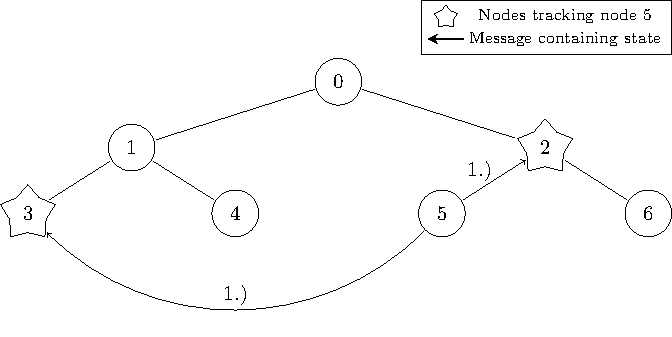
\includegraphics[width=\textwidth]{img/state-exchange/pub_sub_exchange.pdf}
      \caption{Use of publish/subscribe pattern to distribute state.}
    \end{subfigure}  
    \newline 
    \begin{subfigure}{\textwidth}
      \centering
      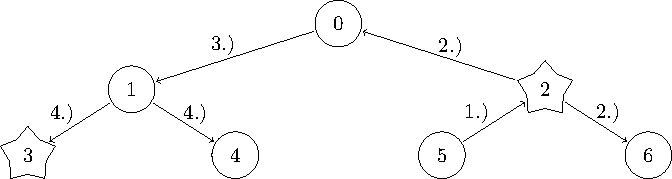
\includegraphics[width=\textwidth]{img/state-exchange/srt_exchange.pdf}
      \caption{Use of SRT to distribute state.}
    \end{subfigure}
    \caption{Message transmissions for state exchange using different messaging patterns.}
    \label{fig:state-exchange}
  \end{figure}

  Nodes gain knowledge about other nodes in two ways. First, a child that selects a new parent sends the parent additional data, such as IP-address, port, and information about its sensors, and is tracked by the parent afterwards. Second, nodes can also actively exchange information about other nodes within the network. This is opposed to the original SRTs in WSNs, where each node simply broadcasts all messages and any node within antenna range can parse the messages. Because of this difference, there is a need for exchange of metadata about nodes within the network. Subsequently, each node maintains local state, where it stores data about several other nodes. It can share its state with other nodes. 
  
  Because the state of a node, e.g. its geospatial location, might change over time, the problem of how to communicate such changes to all interested nodes arises. The way a node propagates its state through the network is critical for the overall messaging overhead. Within a WSN-SRT, nodes route queries and results through the tree and leverage local broadcast, e.g. by message-snooping (see Section~\ref{Semantic Routing Trees}). In the fog, with the ability to address nodes directly, communication patterns are not limited to broadcast. Nodes in the fog can directly propagate changes of their own state through a publish/subscribe pattern, where all interested nodes subscribe to the state of a node. Another variant for state exchange is that nodes do not use a publish/subscribe pattern, but the existing routing tree to limit direct communication and use the existing routing structure instead. Figure~\ref{fig:state-exchange} illustrates how changes of state propagate with both publish/subscribe and use of the SRT, respectively. When using the SRT for propagation, children send their parents updates if their own state changes, and parents forward the data up to their respective parents as well as down to their children, so that all nodes eventually receive the changed state once. If the receiving nodes track the node whose state changed, they update the data. Otherwise, they discard the message. We note here that the intent for SRTs is not metadata exchange and that we do not see an inherent benefit of using a SRT for metadata exchange. In contrary, sending all state changes through the whole SRT induces unnecessary overhead and does not leverage the ability to directly address remote nodes. Therefore, we decide for a publish/subscribe messaging pattern.

  \begin{algorithm}[!h]
    \SetAlgoLined
    \SetKwInOut{Input}{Input}
    \SetKwInOut{Output}{Output}
    \SetKw{Request}{request}
    \SetKw{From}{from}
    \SetKw{Receive}{receive}

    \Input{find-better-parent request}
    \KwData{curr\_dist = distance to current parent \\ 
    \hspace{3.1em}lat = requesting node's latitude \\
    \hspace{3.1em}lon = requesting node's longitude \\
    \hspace{3.1em}pos = (lat,lon)}
    \Output{new parent for requester}
    \BlankLine    
    \Begin{
        best\_dist = INTEGER\_MAX\;
        best\_idx = -1\;        
        \BlankLine
        \tcp{find best parent locally}
        \For{child : self.children}{
            dist = euclidean\_distance(pos, child\_pos)\;
            \If{dist $<$ best\_dist}{
                best\_dist = dist\;
                best\_idx = children.current\_idx\;
            }
        }
        \BlankLine
        \Request random\_sibling \From self.parent\;
        \Receive best\_rand, best\_rand\_dist \tcp{best child from random sibling and requesting node's distance to best child}
        \BlankLine
        \uIf{best\_rand\_dist $<$ best\_dist}{
            \Return{best\_rand, best\_rand\_dist}
        }
        \Else{
            \Return{children[best\_idx], best\_dist}
        }
    }
    \caption{Parent selection at requesting node's grandparent}
    \label{alg:parent-selection}
  \end{algorithm}

  \begin{figure}[t] 
    \centering
    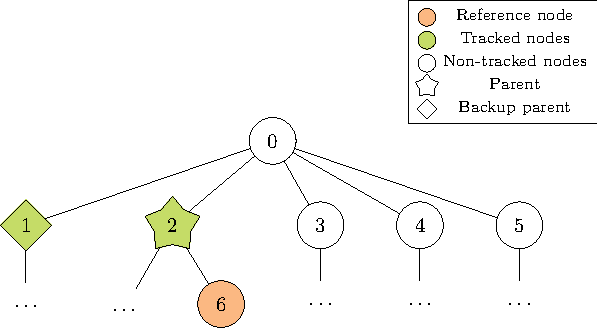
\includegraphics[]{img/specific-srts/tracking-policy/tracking_policy.pdf}
    \caption{Tracking policy: Node 6 tracks the green nodes.}
    \label{fig:srt-tracking-policy}
  \end{figure}  

  If each node keeps track of several other nodes, the question arises which remote nodes each node should track. The naive approach of every node tracking all nodes in the network would likely introduce too much message-transmission overhead. To achieve fast recovery from failure as well as a clustered SRT, every node only needs information about three categories of nodes. First, all nodes need information such as subtree-range about their children, and should thus track all children. Second, a node must know its parent’s tree-attribute value to determine its proximity to the parent. Third, there must be at least one backup, which ideally is the second best parent candidate, for the case of a parent failure. Figure~\ref{fig:srt-tracking-policy} illustrates our proposed tracking policy. 
  
  \begin{figure}[t]
    \centering
    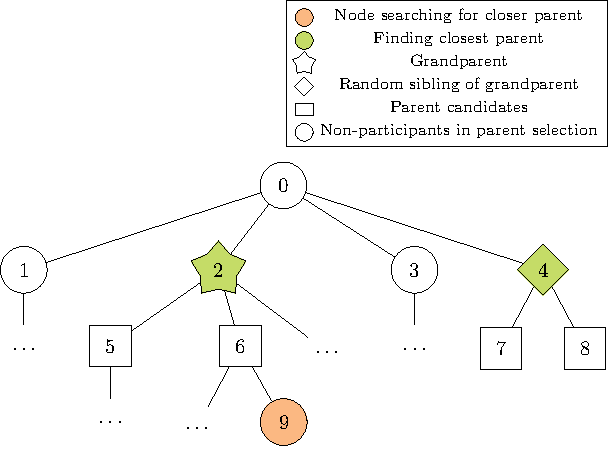
\includegraphics[]{img/specific-srts/parent-selection/parent_selection.pdf}
    \caption{Overview of the participating nodes in parent selection.}
    \label{fig:srt-parent-selection}
  \end{figure}

  Following Section~\ref{Adaption of Semantic Routing Trees to the Fog}, the ideal parent has a close tree-attribute and is closer to the inner edge than its children. To achieve that, we propose the following parent selection algorithm: triggered by events such as a change in its own or the parent’s tree-attribute, a node initializes parent selection. It first sends a message to its parent that contains the node’s tree-attribute distance\footnote{The notion of \textit{distance} is based on the specific tree-attribute. In a SRT based on the location attribute, distance could mean \textit{euclidean distance}.} to the current parent. The parent forwards the message to its parent, i.e. the requesting node’s grandparent. The grandparent, tracking all its immediate descendants, computes the distance of each child to the requesting grandchild. The grandparent additionally forwards the parent-selection-request to a random sibling. This is to enlarge and broaden the set of potential parents for the requesting nodes. After the grandparent has received the closest parent from the random sibling, it selects the best parent out of all candidates, now including all its children and the candidate from the random sibling. Finally, the grandparent forwards the new parent immediately to the grandchild, which subsequently selects it as its new parent. We formalize the approach in Algorithm~\ref{alg:parent-selection}. This approach ensures a optimal parent selection while storing minimal state, with the potential downside of many message transmissions. If the grandparent has many children, which implies many grandchildren, computation of an optimal parent for every grandchild can become costly in terms of message exchanges. Figure~\ref{fig:srt-parent-selection} illustrates the nodes participating in parent selection. For further evaluation of the transmission overhead we refer to Section~\ref{Evaluation}.
  
\section{Tree Construction and Maintenance}\label{Tree Construction and Maintenance}  
  \begin{figure}[bh]         
    \centering
    \begin{subfigure}{0.8\textwidth}
      \centering
      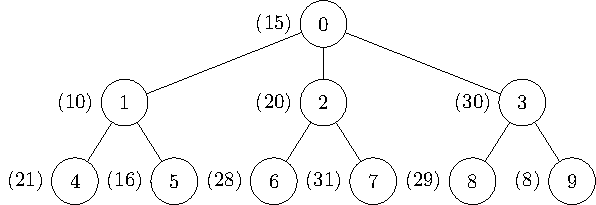
\includegraphics[width=\textwidth]{img/specific-srts/startup/startup_1.pdf}      
      \caption{SRT immediately after start-up}
    \end{subfigure}
    \newline 
    \begin{subfigure}{0.8\textwidth}
      \centering
      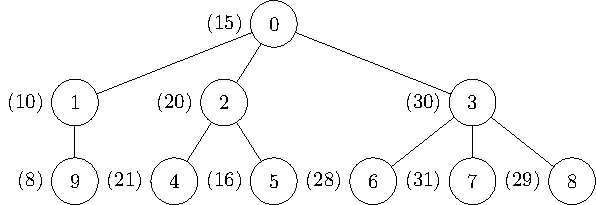
\includegraphics[width=\textwidth]{img/specific-srts/startup/startup_2.pdf}
      \caption{SRT after parent selection}
    \end{subfigure}
    \caption{Behaviour of the SRT after start-up.}
    \label{fig:srt-startup}
  \end{figure}

  The geo-spatial location of nodes is of great importance for organizing the fog, because the idea of the fog layer is to place computational power in close physical proximity to the data sources. Therefore, we argue that all systems using SRTs must have a tree over the location attribute as the initial SRT. To ease the process of creating the location-based initial SRT, each node needs the network address of a parent at start-up. Starting from there, nodes can exchange data and start tracking each other according to the tracking policy. Because a node’s position can change over time, we propose an iterative approach to tree maintenance, where different events trigger the parent selection process: tree-attribute change  at the parent, at the node itself, and parent failure. Because of the minimal information that each node stores locally, it has no information about attribute changes of its parent's siblings, which could become best parent-choices when their tree attribute changes. To improve the quality of the tree in this scenario, children could either send a parent selection message periodically, or attribute changes in higher level nodes could trigger all nodes of the below level to initialize parent selection.
  
  We propose to also leverage the importance of location when constructing new SRTs. Our approach here is to start every new tree based on the current location-tree. In WSNs, nodes that are in close physical proximity to each other can have correlations between other attributes, such as brightness or temperature of the environment~\cite{madden_tinydb:_2005}. If there is such a correlation between location and other attributes, e.g. temperature or brightness, starting a new tree based on location saves message transmissions. From this tree, nodes start the aforementioned iterative approach of switching parents and updating attribute ranges. Figure~\ref{fig:srt-startup} illustrates the behaviour of the SRT after start-up, where nodes switch parents if there is a candidate with a closer tree-attribute.